\section{Première formulation robuste}
\subsection{Modèle}

Afin de prendre en compte les erreurs sur les facteurs d'amplification $x_i$, nous utilisons les valeurs maximales des variations possibles de $\hat{D(\theta)}$\\
Nous imposons que malgré ces variations nous restons dans les intervalles voulus. On transforme par exemple la première contrainte $D(\theta)\leq \epsilon$ :
\begin{eqnarray*}
d(\theta)^T (x.*(1+\ksi)) \leq \epsilon \\ 
d(\theta)^T (x.*\ksi) \leq \epsilon- d(\theta)^T x \\
\end{eqnarray*}
Comme nous cherchons à ce que notre optimum soit valable dans le pire cas, c'est-à-dire celui où
En imposant $|D(\theta)| + \sum_{i=1}^{n} | \tau x_i d_i(\theta)\leq \epsilon $ on est sur que . On traduit de la même manière les contraintes sur $\mathcal{P}$ comme $|D(\theta)-1| + \sum_{i=1}^{n} |\tau x_i d_i(\theta)|\leq \epsilon $ . 
Pour notre problème échantillonné et linéaire, il nous faut donc introduire $n$ variables $v_i$ (associées à chaque $\theta$ échantillonné) correspondant aux valeurs absolues des $\tau d_i(\theta)$. On a alors le modèle : 
\begin{align}
|D(\theta)| + \sum_{i=1}^{n} v_i & \leq  \epsilon & \forall i \in \mathcal{S} \\
|D(\theta)-1| + \sum_{i=1}^{n}v_i & \leq  \epsilon & \forall i \in \mathcal{P} \\
\tau x_i d_i(\theta) & \leq  v_i \\
-\tau x_i d_i(\theta) & \leq  v_i 
\end{align}

\subsection{Analyse des résultats}
Les figures \ref{fig:D-ModRobust1}, \ref{fig:D-ModRobust1-test3RobTau001} et \ref{fig:D-ModRobust1-test3RobTau01} montrent les résultats obtenus pour différentes valeurs de $\tau$ (dans le modèle ainsi que dans les perturbations). Ici les $x$ sont conçus pour mieux résister en cas de perturbations. Un récapitulatif des résultats pour les différents modèle est donné à la table \ref{table:Recap}. Notons que ces modèles sont bien plus performant que le modèle de base. En effet le $\epsilon$ augmente très peu $2\%$ dans le modèle de base à $2.8\%$ ou $3.3\%$ dans le modèle robuste; tandis que la robustesse s'améliore nettement.\\
\begin{itemize}
\item Dans le cas $\tau = 0.001$, on constate une augmentation du $\epsilon$ par rapport au modèle de base. Les erreurs pour les $x_i$ perturbés sont cependant bien moindre. On constate également que les erreurs pour le modèle $x_i$ perturbés avec ue perturbation de l'ordre de $\tau=0.001$ sont moindre que dans le modèle avec $\tau=0.01$.\\ 
 \item Dans le cas $\tau = 0.01$, on constate toujours une augmentation du $\epsilon$ par rapport au modèle de base et au modèle où $\tau = 0.001$. Les erreurs pour les $x_i$ perturbés sont moindre que dans le modèle $\tau=0.001$ pour des perturbations de l'ordre de $\tau = 0.01$.
\end{itemize}
Bref, les deux modèle robustes se comporte le mieux pour les perturbations auxquelles ils sont sensés résister.

\begin{figure}[h!]
  \centering
  \begin{subfigure}[b]{0.45\textwidth}
  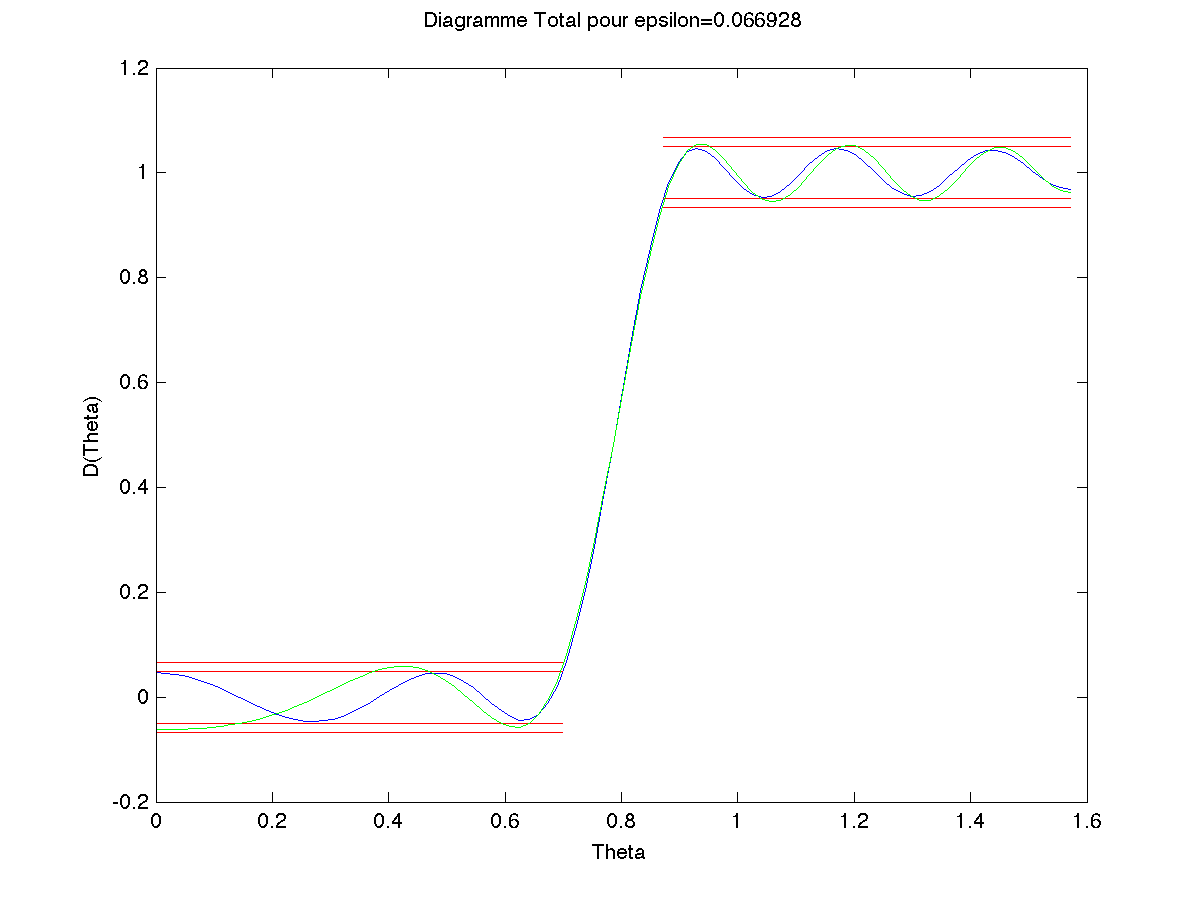
\includegraphics[width=\textwidth]{D-ModRobust1.png}
  \caption{$D(\theta)$ pour le modèle $\tau = 0.01$ (en vert) et $\tau = 0.001$ (en bleu) et $x$ non-perturbé.}
  \label{fig:D-ModRobust1}
  \end{subfigure}
  ~ 
 \begin{subfigure}[b]{0.45\textwidth}
  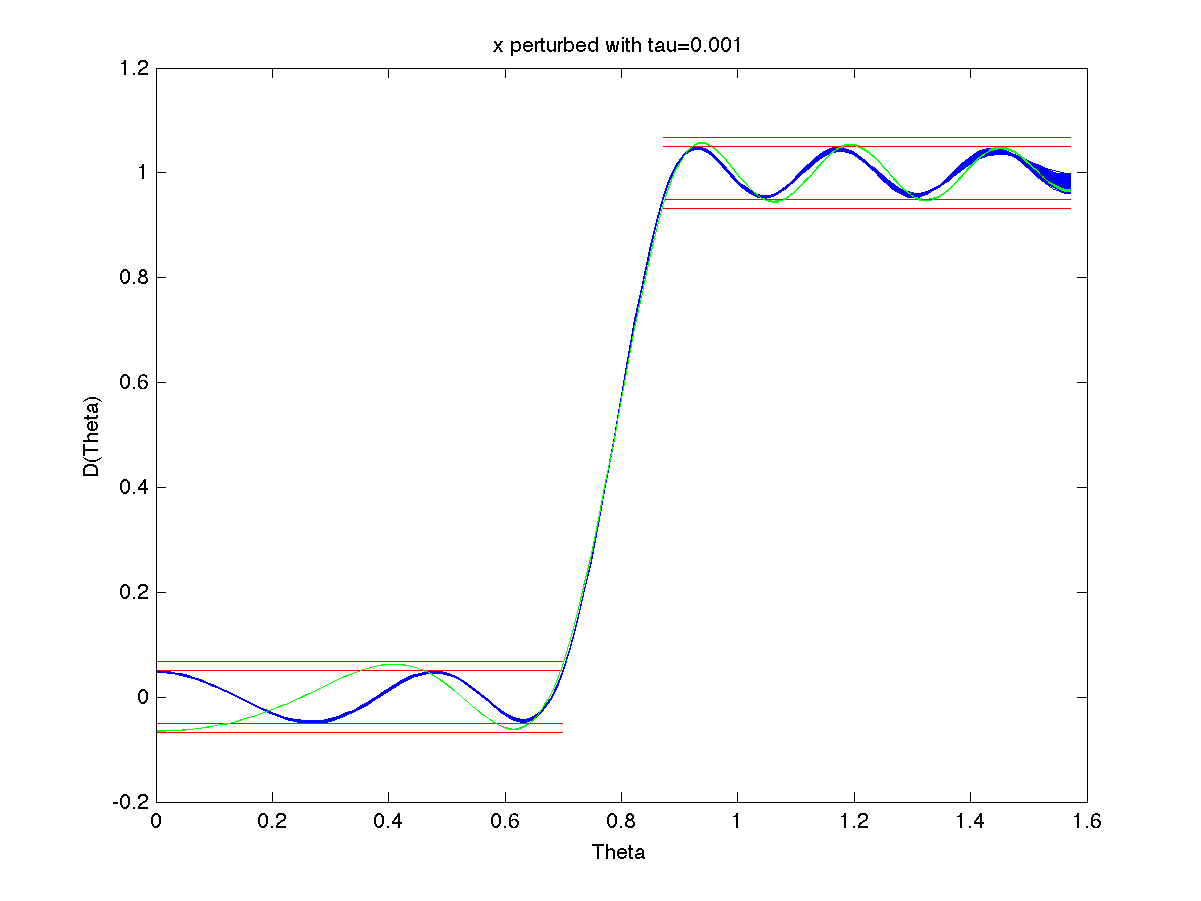
\includegraphics[width=\textwidth]{D-ModRobust1-test3Rob001.png}
  \caption{$D(\theta)$ pour une perturbation de $\tau = 0.001$ sur les $x$ (en vert pour un modèle de $\tau=0.01$ en bleu pour $\tau=0.001$).}
  \label{fig:D-ModRobust1-test3RobTau001}
  \end{subfigure}
  \begin{subfigure}[b]{0.45\textwidth}
  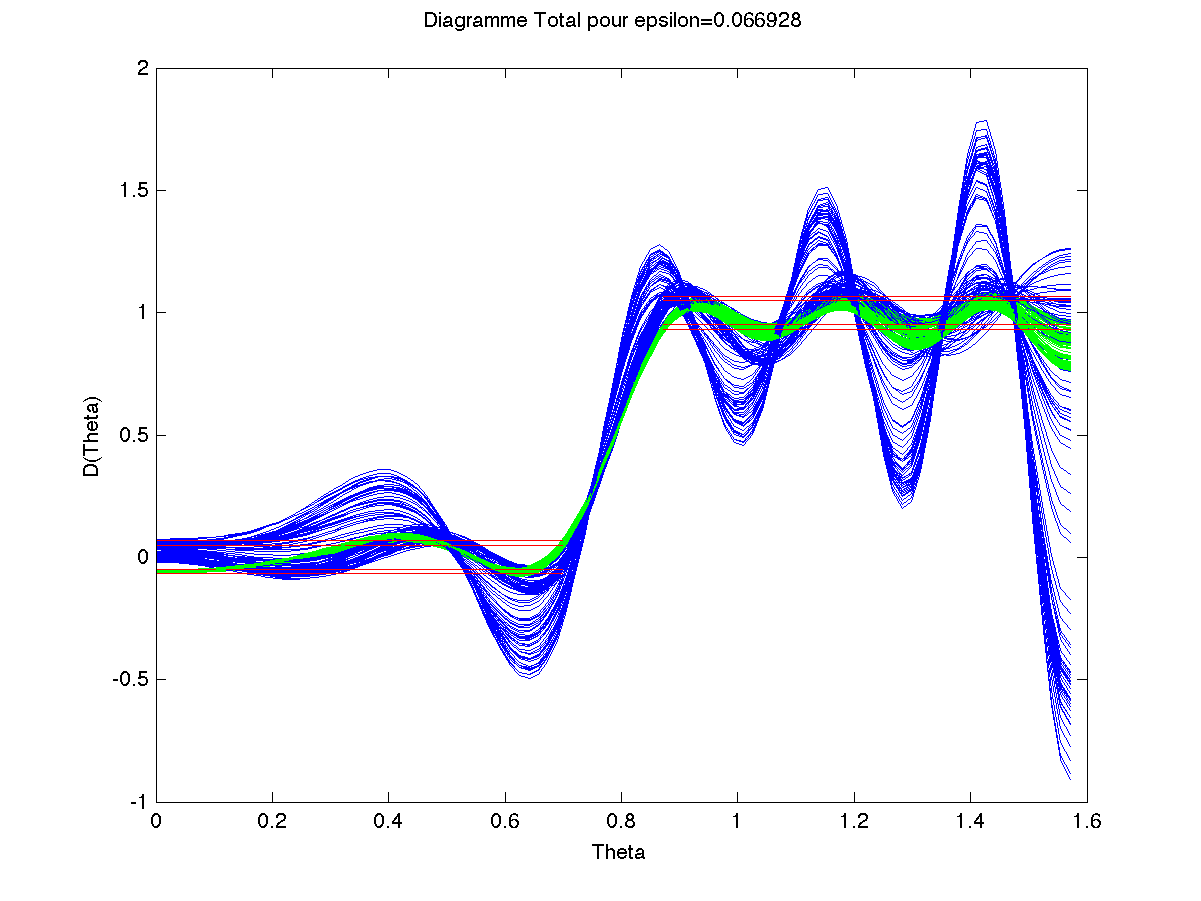
\includegraphics[width=\textwidth]{D-ModRobust1-test3Rob01.png}
  \caption{$D(\theta)$ pour une perturbation de $\tau = 0.01$ sur les $x$ (en vert pour un modèle de $\tau=0.01$ en bleu pour $\tau=0.001$).}
  \label{fig:D-ModRobust1-test3RobTau01}
  \end{subfigure}
  \caption{}
  \end{figure}

\begin{table}
\centering
\begin{tabular}{c|c|ccc}
 & & & \textbf{Erreurs pour : } &\\
 & $\epsilon$ & $x_i$ non-perturbés & $x_i$ perturbés ($\tau=0.001$) & $x_i$ perturbés ($\tau=0.01$) \\
 \hline
Modèle de base & $2\%$ & 0.0185 & 5.3977 & 47.9054 \\
Modèle robuste 1 ($\tau=0.001$) & $5.0 \%$ & 0.0398 & 0.0479   & 0.2024 \\
Modèle robuste 1 ($\tau=0.01$)  & $6.7 \%$ & 0.0505 & 0.0508& 0.0628 \\
\end{tabular}
\caption{Récapitulatif des résultats des erreurs et de la borne maximal $\epsilon$ obtenus pour les différents modèles et les différents types de perturbations.}
\label{table:Recap}
\end{table}